\section{$\phi$-meson analysis} 
\subsection{Particle reconstruction}
\subsection{Acceptance and efficiency}
\subsubsection{Acceptance}

\begin{figure}[h]
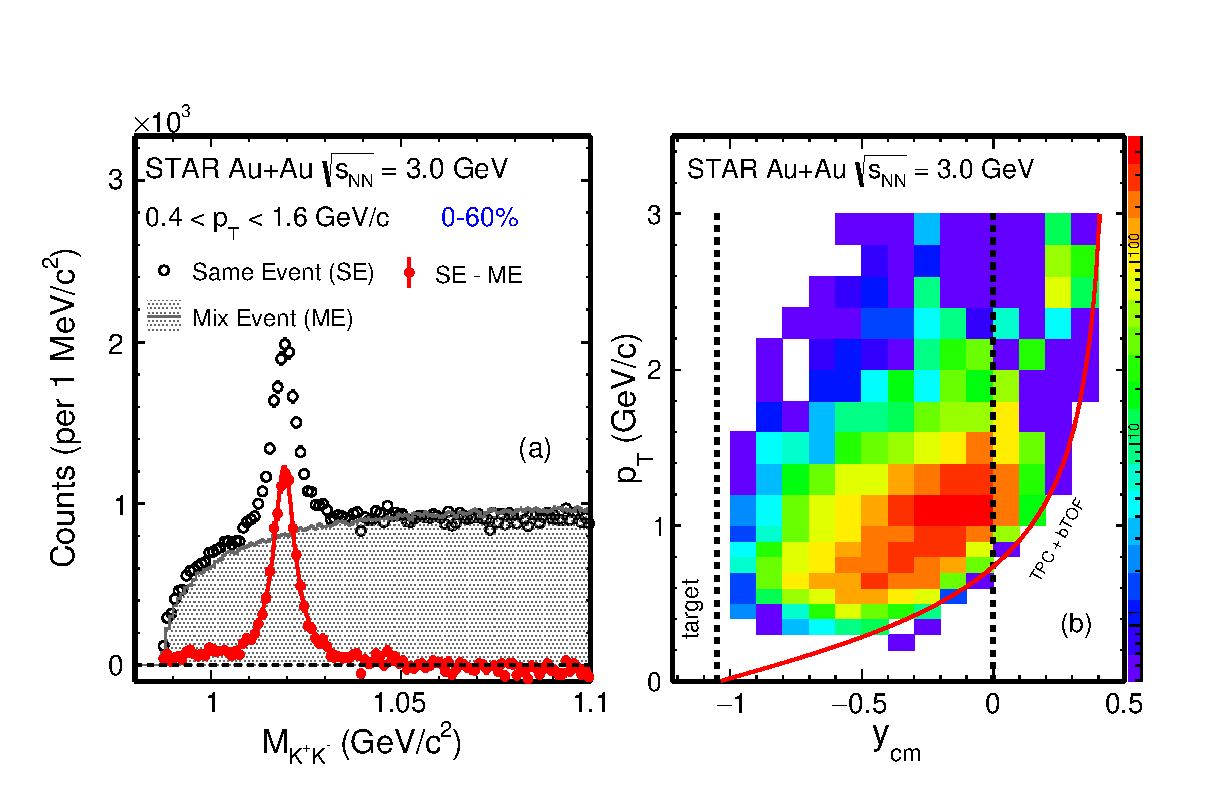
\includegraphics[width=0.85\linewidth]{chapterY/fig/fig1_signal.eps}
  \caption{(a) Invariant mass of $K^+K^-$ pairs in 0-60\% centrality and 0.4--1.6\,GeV/$c$ for the total inclusive yield. (b) The reconstructed $\phi$-meson acceptance $p_T$ vs. rapidity in the center-of-mass frame ($y_{\rm cm}$).}
\label{phiSignal}
\end{figure}

Fig.~\ref{phiSignal} shows the invariant mass of $K^+K^-$ pairs for total inclusive one. Black open circles represent the same-event (SE) unlike-sign (US) distributions. Grey shaded histograms represent the mix-event (ME) US distributions that are used to estimate the combinatorial background. The red solid circles depict the $\phi$-meson signals obtained by subtracting the ME combinatorial background from the SE distributions. (b) The reconstructed $\phi$-meson acceptance $p_T$ vs. rapidity in the center-of-mass frame ($y_{\rm cm}$).


\subsubsection{Efficiency corrections}

\begin{figure}[h]
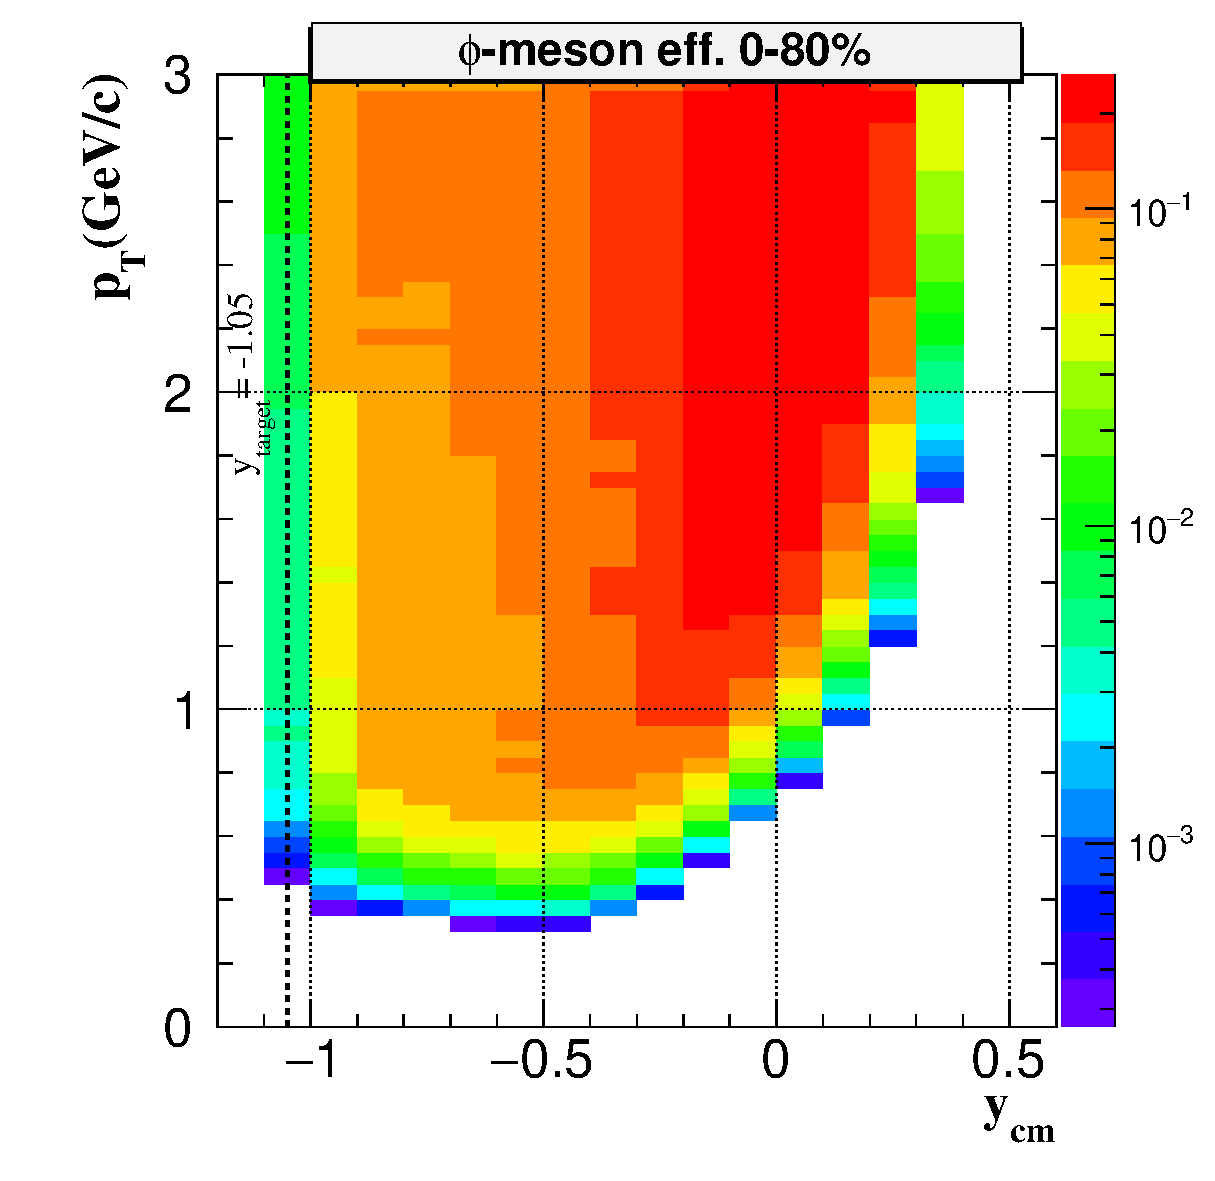
\includegraphics[width=0.6\linewidth]{chapterY/fig/2effAll_rap_0.eps}
\caption{Reconstruction efficiency of $\phi$, as a function of $y$ and $p_{\rm{T}}$ at $\sqrt{s_{NN}}$ = 3 GeV.}
\label{phi_2Deff}
\end{figure}

Fig.~\ref{phi_2Deff} shows the 2D y vs $p_T$ $\phi$-meson reconstruction efficiency used as a re-weight factor for the flow analysis to consider the acceptance effect.


\subsection{$v_1$ and $v_2$ extraction and systematic uncertainties}

\subsubsection{$v_1$}

$\phi$-meson was divided into 6 $\phi$-$\Psi_{1}$ range as shown in Fig.~\ref{phi_v1} from [0, $\pi$], for each range, after the combinatorial background subtracting, a breit-wigner function was used for fitting to extract the raw counts in each individual range. After that, the raw counts was fitted with the function \ref{equ:equation_v1} to extract the raw $v_1$ as shown in Fig.~\ref{phi_v1_fit}. After correct the event plan resolution, the corrected $v_1$ was obtained.

\begin{equation}
  \frac{dN}{d($\phi$-$\Psi_{1}$)} \propto 1+2$v_1$cos($\phi$-$\Psi_{1}$),
\label{equ:equation_v1}
\end{equation}


\begin{figure}[h]
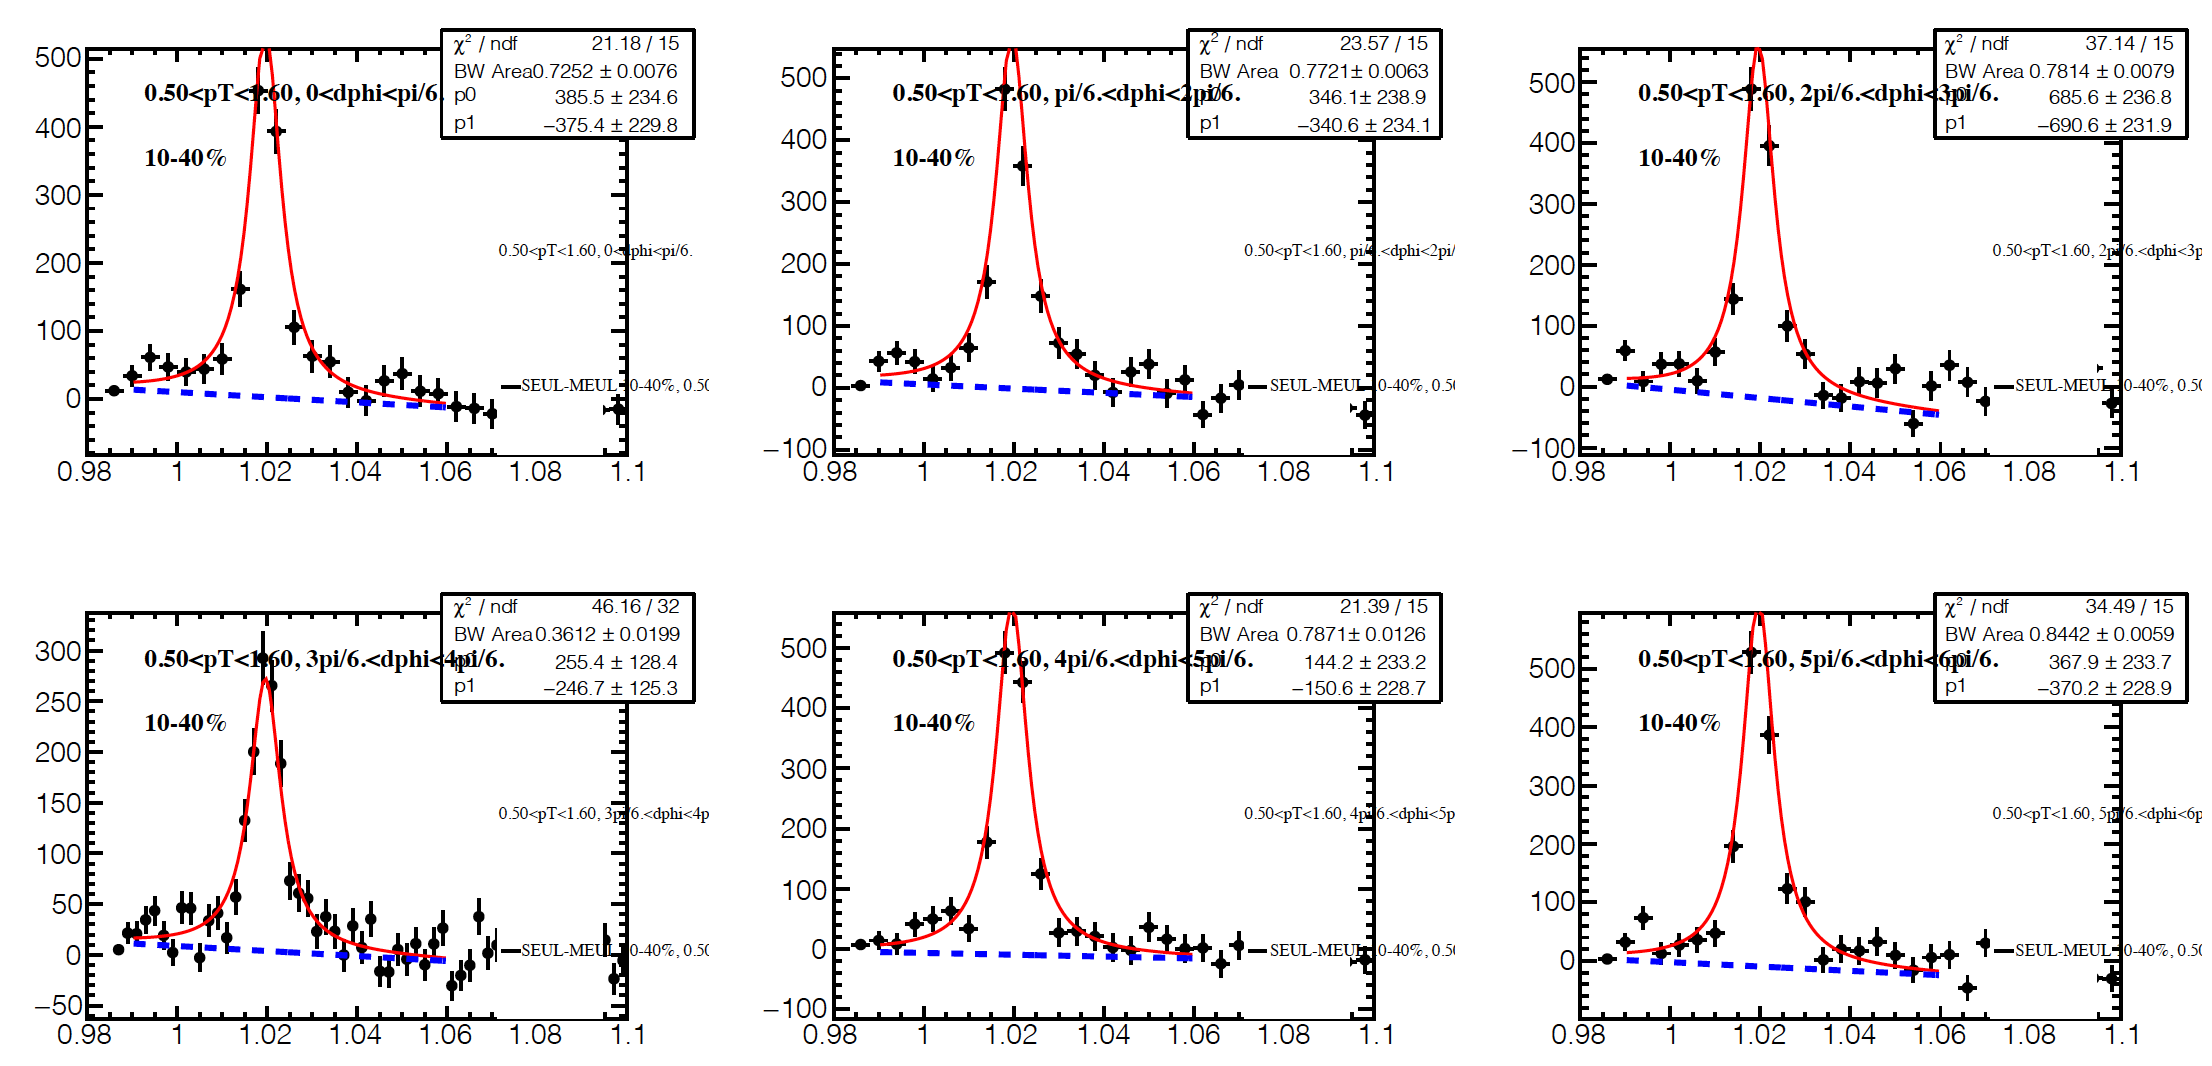
\includegraphics[width=0.98\linewidth]{chapterY/fig/phi_invEP_v1_10_40.png}
\caption{$\phi$-meson signals in several different $\phi$-$\Psi$ range.}
\label{phi_v1}
\end{figure}

\begin{figure}[h]
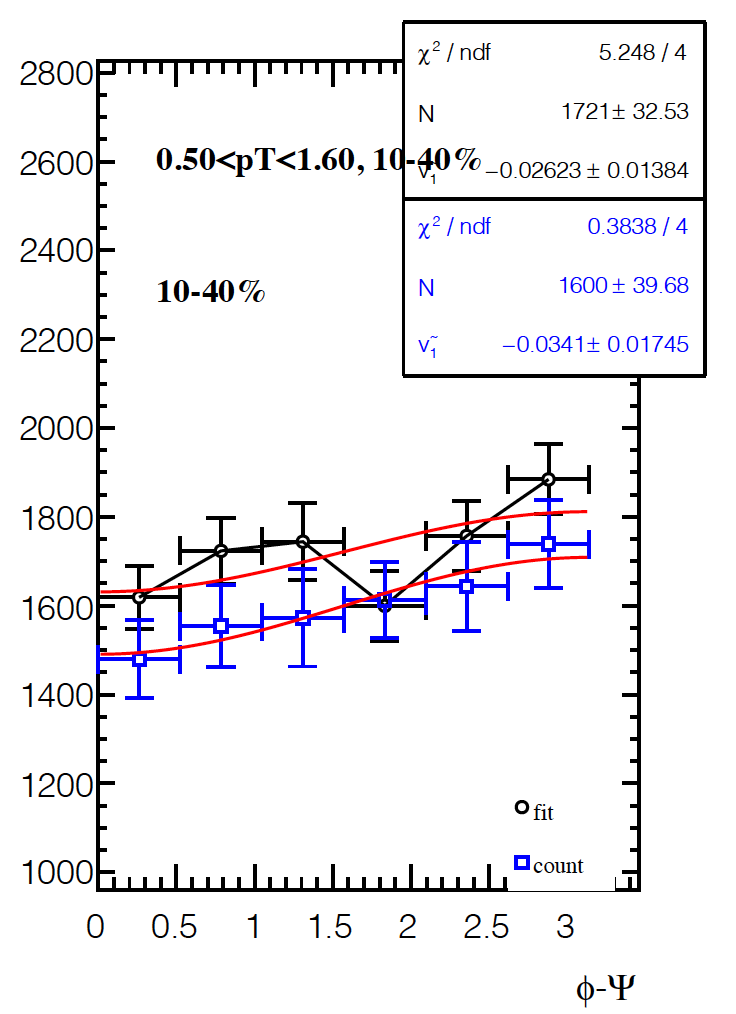
\includegraphics[width=0.55\linewidth]{chapterY/fig/phi_invEP_v1_10_40_fit.png}
  \caption{$\phi$-meson raw counts vs. $\phi$-$\Psi$, fitted with the function to extract the raw v1.}
\label{phi_v1_fit}
\end{figure}

Fig.~\ref{phi_dv1dy} shows an example of the extracted $\phi$-meson $v_1$ along with the rapidity dependence. A linear function which cross (0,0) was used to fitting and obtain the $dv_{1}$/$dy$ slop.

\begin{figure}[h]
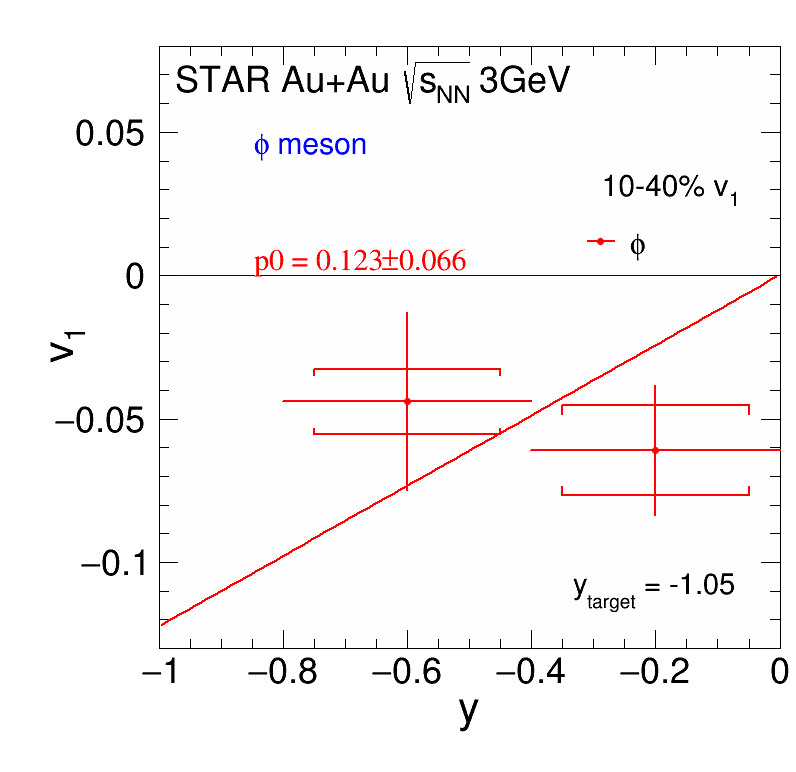
\includegraphics[width=0.49\linewidth]{chapterY/fig/fig1_phi_v1Slop1_10_40.png}
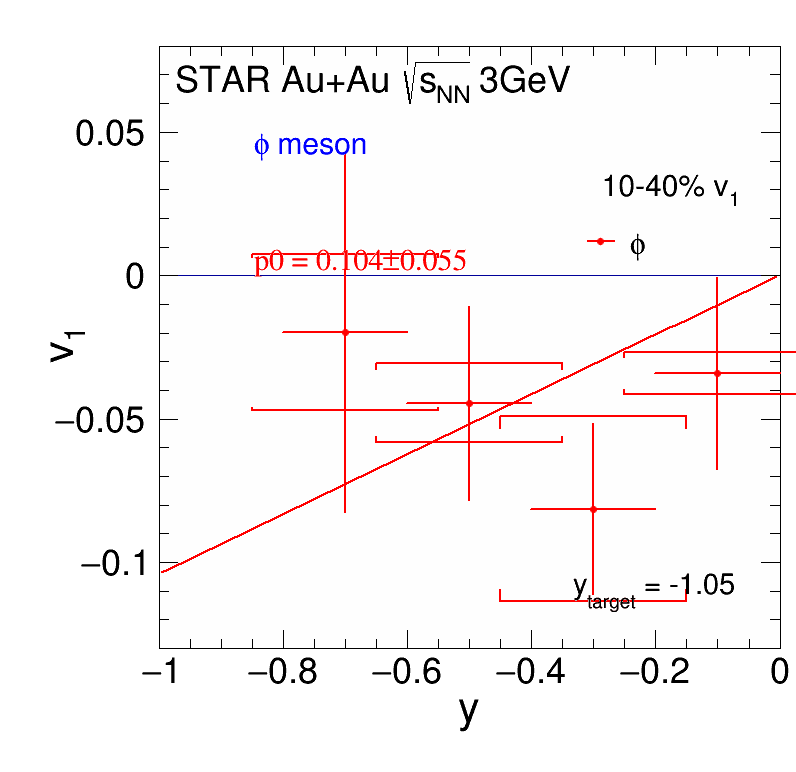
\includegraphics[width=0.49\linewidth]{chapterY/fig/fig1_phi_v1Slop11_10_40.png}
  \caption{$\phi$-meson $v_1$ vs. y, fitted with a linear function cross (0,0).}
\label{phi_dv1dy}
\end{figure}

\subsubsection{$v_2$}

Similar as the $v_1$ analysis, the $\phi$-meson was divided into different $\phi$-$\Psi_{1}$ range and fitted to extract the raw counts and raw $v_2$ as shown in Fig.~\ref{phi_v2} and Fig.~\ref{phi_v2_fit}. The corrected $v_2$ also need to correct the second order event plan resolution which is the same as discussed in the previous section for $\pi$, K and p.

\begin{figure}[h]
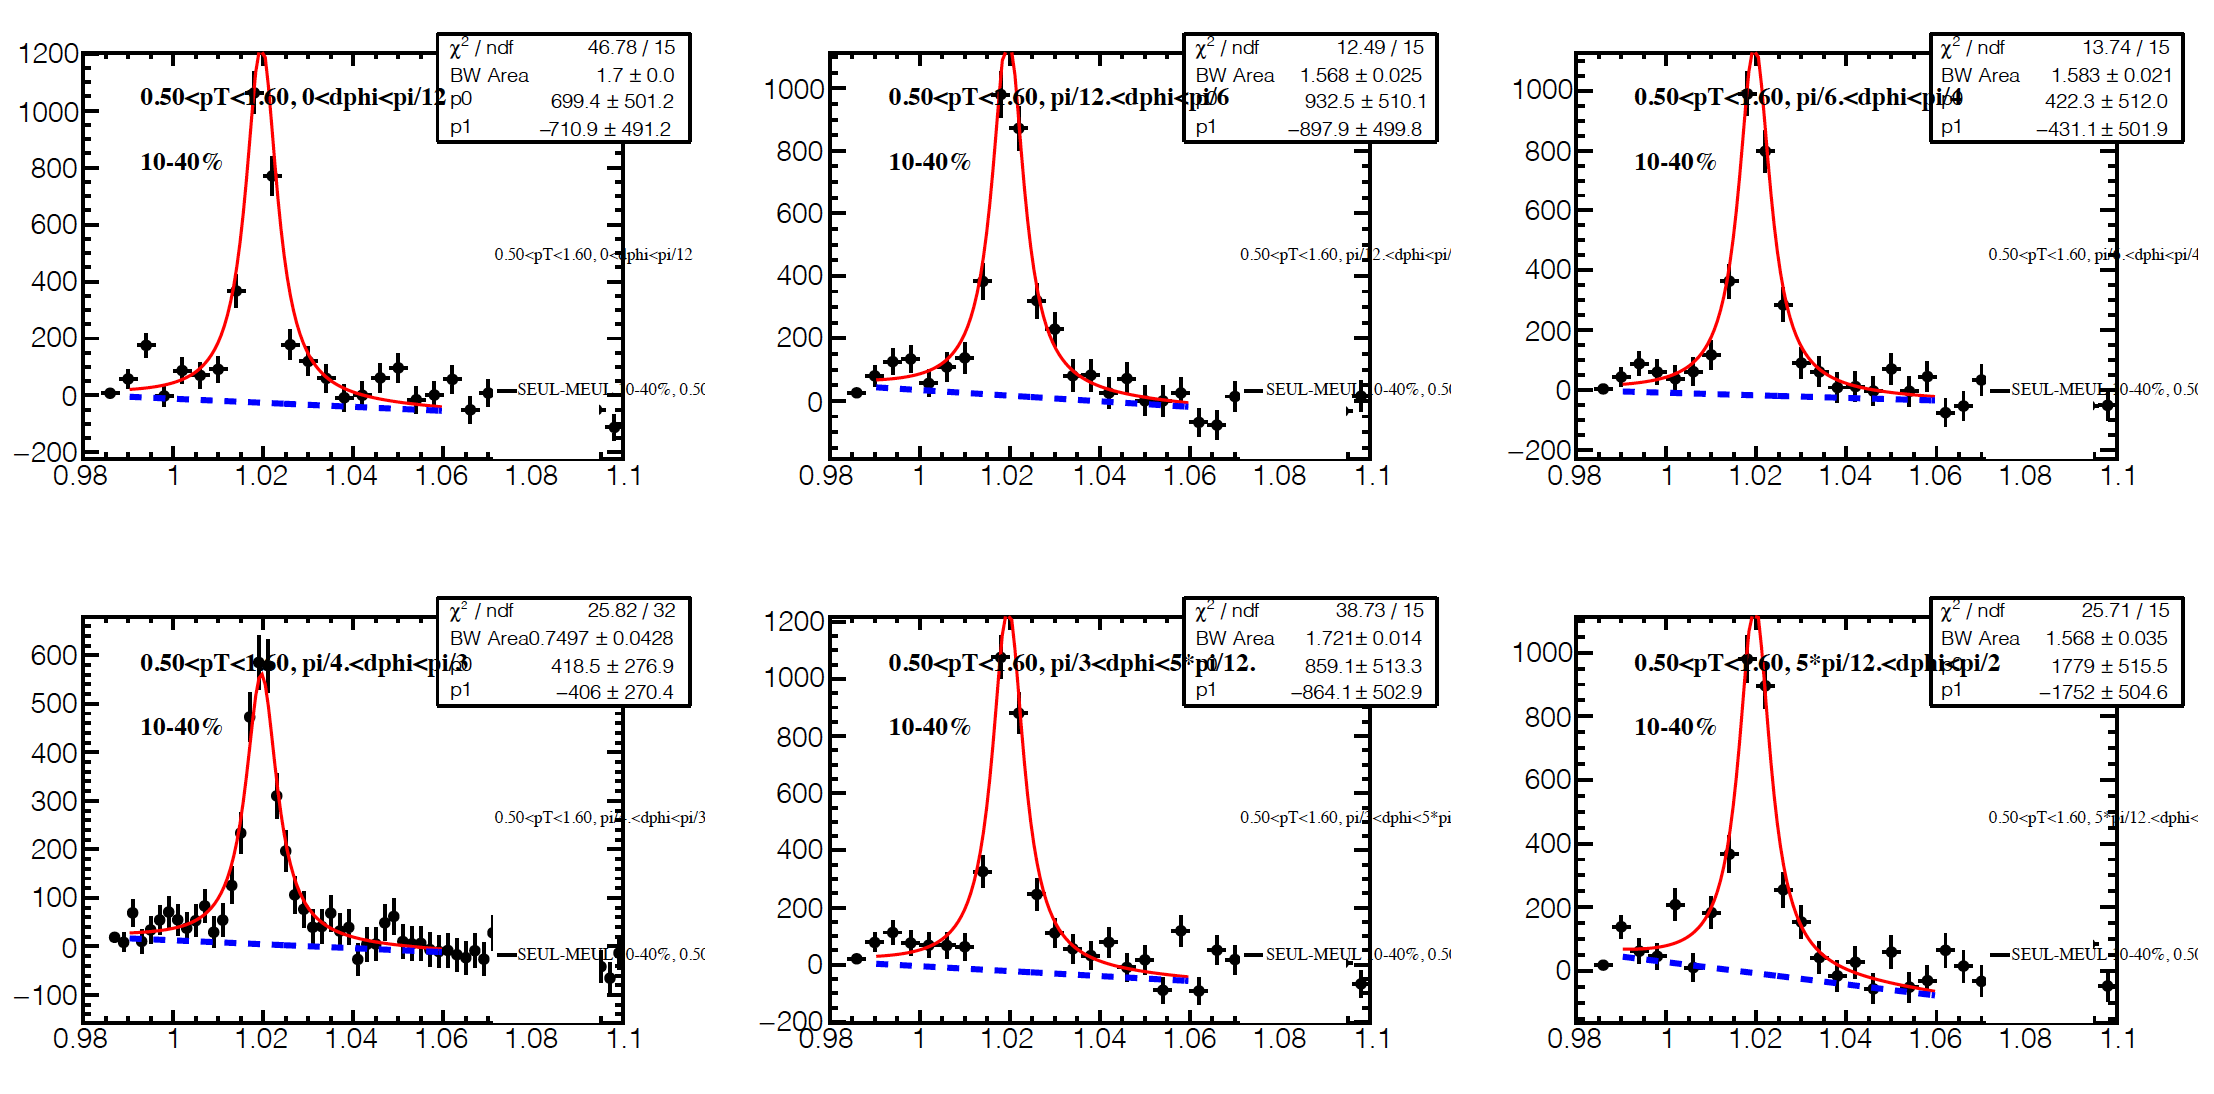
\includegraphics[width=0.98\linewidth]{chapterY/fig/phi_invEP_v2_10_40.png}
\caption{$\phi$-meson signals in several different $\phi$-$\Psi$ range.}
\label{phi_v2}
\end{figure}

\begin{figure}[h]
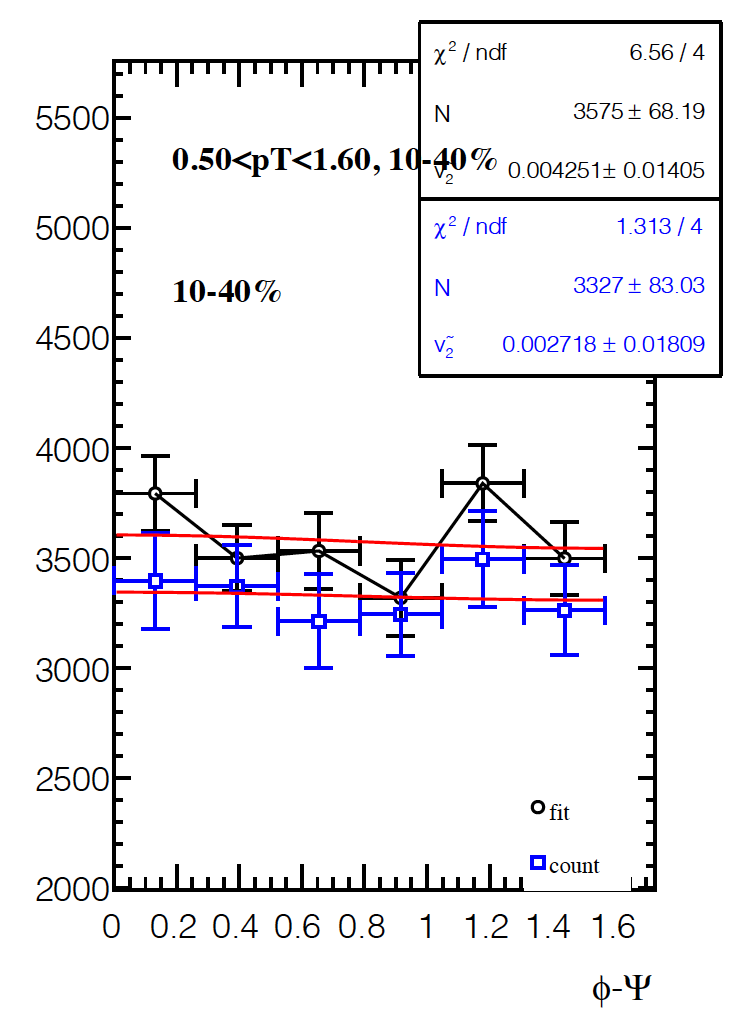
\includegraphics[width=0.45\linewidth]{chapterY/fig/phi_invEP_v2_10_40_fit.png}
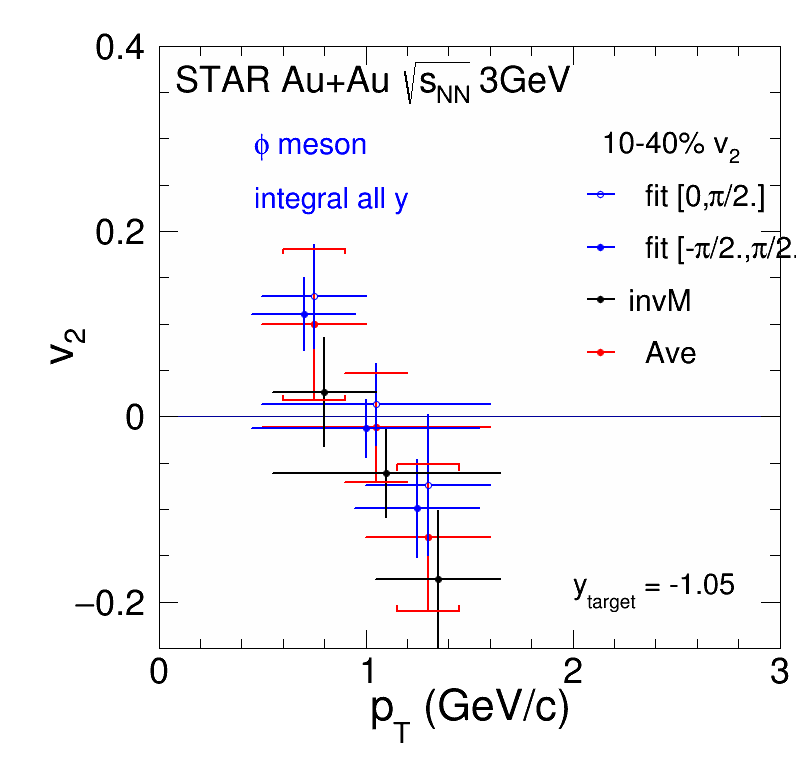
\includegraphics[width=0.49\linewidth]{chapterY/fig/fig1_phi_v2_10_40.png}
  \caption{(left) $\phi$-meson raw counts vs. \phi$-$\Psi for selected $p_T$ as one example, fitted with the function to extract the raw v2. (right) $\phi$-meson $v_2$ vs. $p_T$, here the three $p_T$ range are from [0.5,1.0],[1.0,1.6],[0.5,1.6].}
\label{phi_v2_fit_pT}
\end{figure}

For the systematic uncertainties, several components were used to evaluate the contribution, basically the same as for the $\phi$-meson spectra analysis: we vary the nHitsFit, dca, n$\sigma_{K}$, 1/$\beta$ for the analysis and we also take different $\phi$-$\Psi_{1}$ fit range for the $v_1$ and $v_2$ extraction and take the difference as the systematic. For each physical variable, since the data precision is not good, we always use the averaged value from all different cuts as the central value to avoid the fluctuations. 

\subsection{Results}
\subsubsection{$v_1$ results for $\phi$-meson}

Fig.~\ref{phi_dv1dy_energy} shows the $\phi$-meson $dv_1/dy$ slop along with the collision energies for the 10-40\% centrality. As see, with the data precision, there is a hint of positive $dv_1/dy$ slop at 3 GeV which is the same trend as $\pi$, K, p, $K_{s}^0$ and $\Lambda$. Fig.~\ref{phi_v2_pT} shows the $\phi$-meson $v_2/n_q$ along with the scaled kinetic momentum $m_T-m_0/n_q$ for the 10-40\% centrality in mid-rapidity. As see, with the data precision, that is really hard to conclude whether the $\phi$-meson follow the NCQ scaling or not.

\begin{figure}[h]
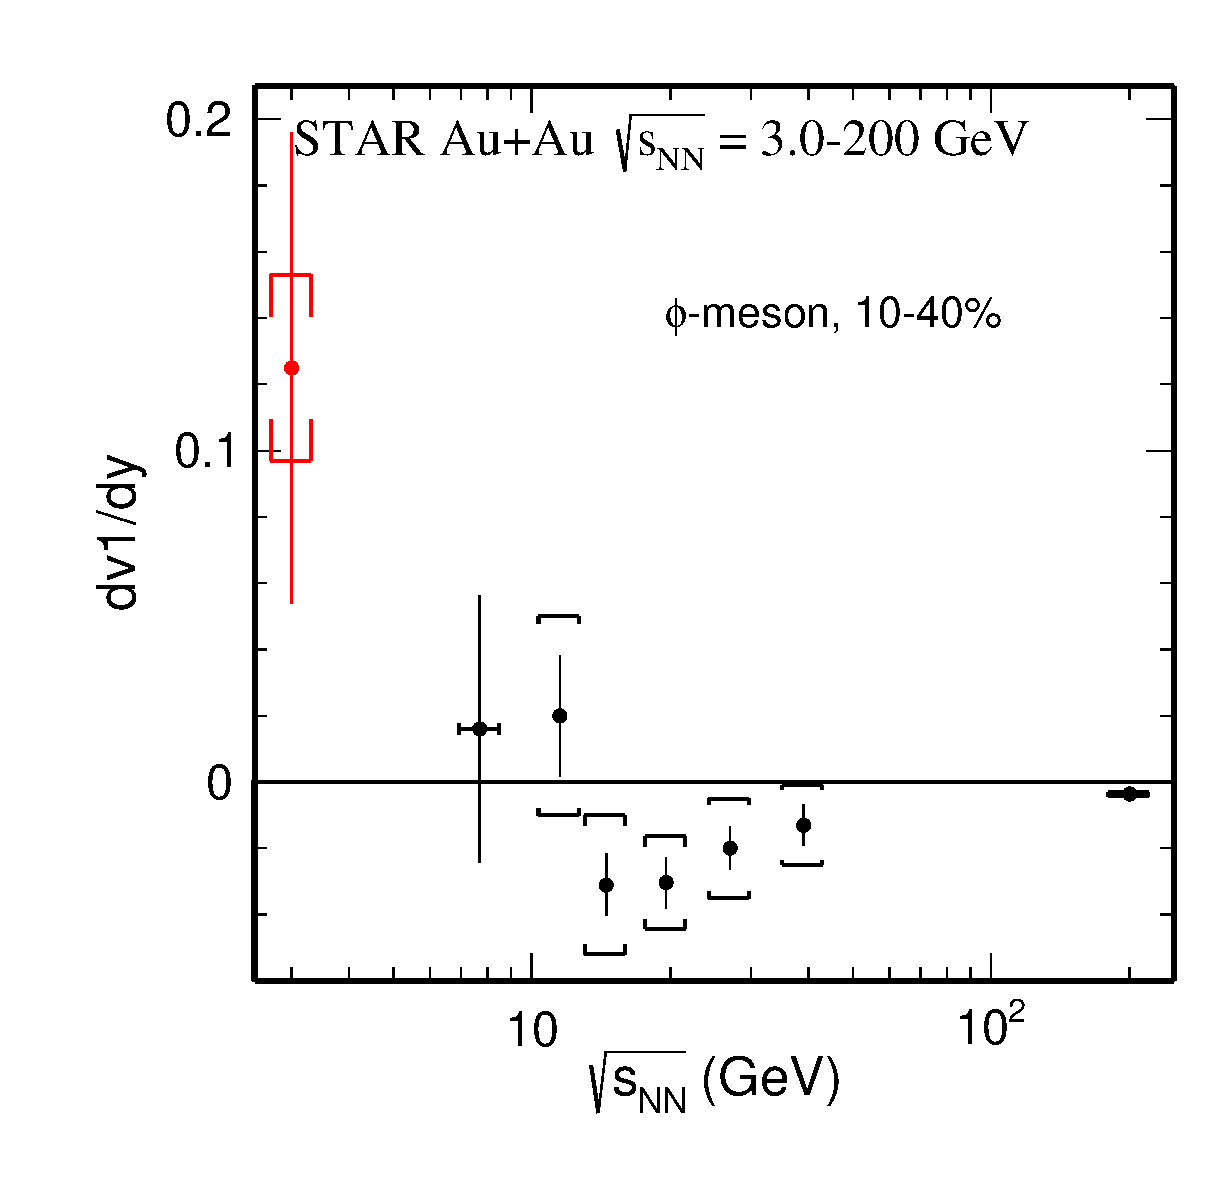
\includegraphics[width=0.6\linewidth]{chapterY/fig/Fffig_dv1_vs_sNN.eps}
\caption{$\phi$-meson d$v_1$/dy slop as a function of collision energies for $10-40\%$ centrality.}
\label{phi_dv1dy_energy}
\end{figure}

\subsubsection{$v_2$ results for $\phi$-meson}

\begin{figure}[h]
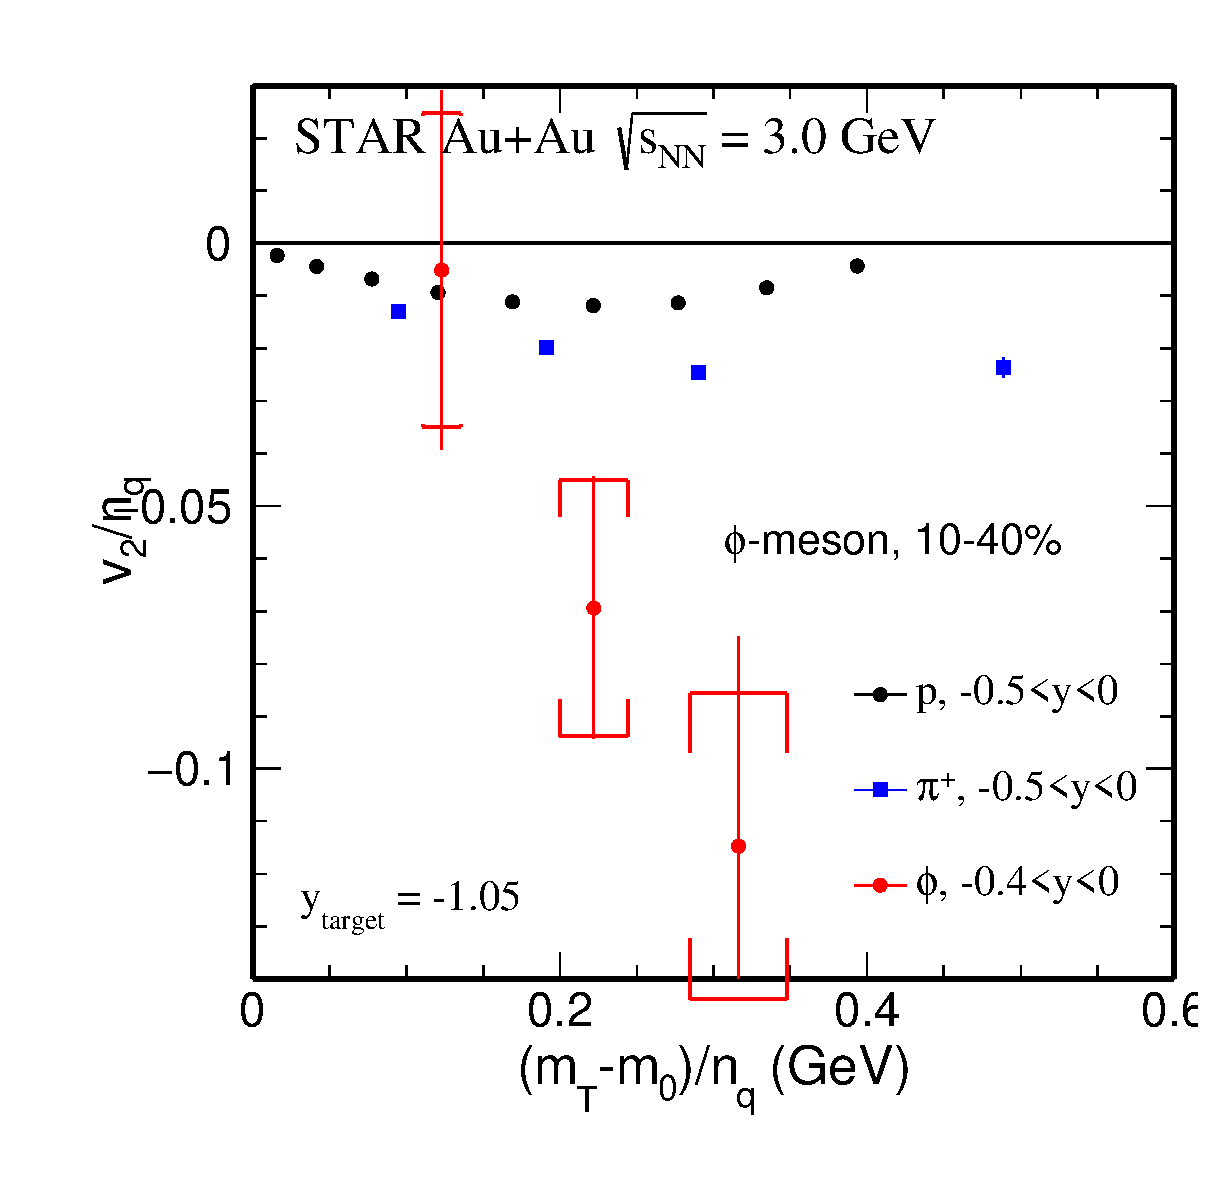
\includegraphics[width=0.6\linewidth]{chapterY/fig/Fffig_v2NCQ_y00p4.eps}
\caption{$\phi$-meson $v_2$/$n_q$ scaling as a function of $m_T-m_0$/$n_q$ for $10-40\%$ centrality and compared with the $\pi$ and p.}
\label{phi_v2_pT}
\end{figure}
